% CAMM 535 Final Project — Report 1 (Single-file LaTeX Template)
% Group 4 — Schwannoma
%
% Part 0 checklist:
%  ✓ Clean, consistent report format
%  ✓ Automatic figure numbering
%  ✓ Proper figure captions (legends) + in-text referencing
%  ✓ Proper citations + references (single .tex file; no .bib)
%
% Compile (recommended):
%   pdflatex report1.tex
%   pdflatex report1.tex

\documentclass[11pt]{article}

% ---------- Page / Layout ----------
\usepackage[margin=1in]{geometry}
\usepackage{setspace}
\setstretch{1.15}
\usepackage{microtype}

% ---------- Fonts & Encoding ----------
\usepackage[T1]{fontenc}
\usepackage[utf8]{inputenc} % keep for pdflatex
\usepackage{lmodern}

% ---------- Figures / Tables ----------
\usepackage{graphicx}
\usepackage{float}          % [H] if you need strict placement
\usepackage{booktabs}
\usepackage{longtable}
\usepackage{array}

% ---------- Captions (Figure Legends) ----------
\usepackage{caption}
\captionsetup{
	font=small,
	labelfont=bf,
	labelsep=period
}
\usepackage{subcaption}
% ---------- References / Hyperlinks ----------
\usepackage[hidelinks]{hyperref}
\usepackage[nameinlink,capitalise,noabbrev]{cleveref}

% ---------- Citations (single-file; no .bib) ----------
% Simple and convenient: manual bibliography with \cite{key}
\usepackage[numbers,sort&compress]{natbib}
% ---------- Code Environment ----------
\usepackage{listings}
\usepackage{xcolor} % often needed by listings
\usepackage{float}  % for [H]
\lstset{
	basicstyle=\ttfamily\small,
	columns=fullflexible,
	keepspaces=true,
	showstringspaces=false,
	showspaces=false,
	showtabs=false,
	tabsize=4,
	breaklines=true,
	breakatwhitespace=false,
	upquote=true
}

% ---------- Title metadata ----------
\title{CAMM 535 Final Project — Report 1\\Group 4: Schwannoma}
\author{
	Member 1: \textit{Alireza Khoeini} \\
	Member 2: \textit{Alireza Noroozi} \\
	Member 3: \textit{Ghada}
}
\date{January 2026}

% ---------- Handy commands ----------
\newcommand{\tool}[1]{\texttt{#1}}
\newcommand{\file}[1]{\texttt{#1}}
\newcommand{\db}[1]{\textbf{#1}}

\begin{document}
	\maketitle
	
	\begin{abstract}
		This report documents data acquisition and the conceptual database design for Schwannoma.
		We integrate multiple biological databases to construct a unified schema linking phenotype-related
		genes, variants, genomic coordinates, proteins, and GEO2R results.
	\end{abstract}
	
	\tableofcontents
	\newpage
	
	% =========================================================
	\section{Part 1 — Disease / Phenotype Introduction}\label{sec:intro}
	Schwannoma is a typically benign, slow-growing peripheral nerve sheath tumor that arises
	from Schwann cells, the glial cells responsible for myelination of peripheral nerves.
	Schwannomas most commonly affect cranial and spinal nerves and are frequently associated
	with the vestibular branch of the eighth cranial nerve, where they are known as vestibular
	schwannomas (also called acoustic neuromas) \cite{review_schwannoma_2020}.
	
	\subsection{Clinical characteristics}
	Clinically, schwannomas usually present as well-circumscribed, encapsulated tumors.
	Symptoms depend on tumor location and size and may include hearing loss, tinnitus,
	balance disturbances, localized pain, or neurological deficits due to nerve compression.
	Vestibular schwannomas represent the most common subtype and account for approximately
	8--10\% of all intracranial tumors \cite{vestibular_epidemiology_2019}.
	Although most schwannomas are sporadic, bilateral vestibular schwannomas are a hallmark
	feature of neurofibromatosis type 2 (NF2), a hereditary tumor predisposition syndrome
	\cite{omim_nf2}.
	\subsubsection{Annual incidence (sporadic vestibular schwannoma)}
	
	Population-based registry data suggest that sporadic vestibular schwannoma (VS) is diagnosed at an annual rate on the order of a few cases per 100{,}000 people. In a recent UK cohort registry study (2013--2016), the mean annual incidence of newly diagnosed VS was reported as \textbf{2.2 per 100{,}000 person-years}, with incidence rising strongly with age and peaking in the \textbf{60--69} year group (about \textbf{5.8 per 100{,}000 person-years}) \cite{FernandezMendez2023}. Consistent with this scale, recent US population-based surveillance (CBTRUS, 2017--2021) reports an age-adjusted incidence rate for \textbf{vestibular schwannoma of 1.52 per 100{,}000} and shows that vestibular schwannoma constitutes the majority of non-malignant nerve sheath tumors in the CNS (Figure~\ref{fig:cbtrus_vs_share}) \cite{Price2024CBTRUS}.
	
	\begin{figure}[t]
		\centering
		\includegraphics[width=0.92\linewidth]{figures/cbtrus_figure12.jpg}
		\caption{CBTRUS (US, 2017--2021): distribution of non-malignant primary brain/CNS tumors by (A) site and (B) histopathology. Panel B highlights that vestibular schwannoma represents a large fraction of nerve sheath tumors. Adapted from \cite{Price2024CBTRUS}.}
		\label{fig:cbtrus_vs_share}
	\end{figure}
	
	\subsection{Biological relevance}
	From a biological perspective, schwannomas provide an important model for studying
	tumor suppressor gene dysfunction and dysregulated cell signaling in glial-derived tumors.
	Schwann cells play a critical role in axonal support and nerve regeneration, and disruption
	of their growth control mechanisms can lead to uncontrolled proliferation.
	Schwannoma cells typically retain a benign histological appearance, yet they can cause
	significant morbidity due to their anatomical location and compressive growth pattern
	\cite{pathology_schwannoma_2018}.
	
	\subsection{Known genetic associations}
	...
	
The most well-established genetic association in schwannoma is loss-of-function mutation
or deletion of the \emph{NF2} gene, which encodes the tumor suppressor protein merlin
(schwannomin). Merlin is a key regulator of contact inhibition and multiple signaling
pathways, including Hippo, PI3K/AKT, and MAPK pathways \cite{merlin_signaling_2021}.
In sporadic schwannomas, somatic alterations of \emph{NF2} are observed in a majority of
cases, while germline mutations are characteristic of patients with NF2-associated disease.
Additional genetic and epigenetic alterations involving pathways related to cytoskeletal
organization and cell adhesion have also been reported, highlighting the molecular
heterogeneity of schwannomas \cite{genomics_schwannoma_2022}.

\begin{figure}[htbp]
	\centering
	\includegraphics[width=0.85\linewidth]{figures/nf2_merlin_pathway.png}
	\caption{\textbf{NF2/merlin signaling pathways in schwannoma development.}
		Merlin regulates multiple growth-control pathways, including Hippo, PI3K/AKT,
		and MAPK signaling. Loss of NF2 function removes growth inhibition in Schwann
		cells and promotes tumor formation. Adapted from \cite{merlin_signaling_2024}.}
	
	\label{fig:nf2_pathway}
\end{figure}

As illustrated in \Cref{fig:nf2_pathway}, disruption of merlin-mediated signaling
removes critical growth-inhibitory signals in Schwann cells.

	\newpage
	% =========================================================
	\section{Part 2: Gene Selection and Variant Retrieval}
	
	\subsection{Step 1: Identification of Schwannoma-Associated Genes Using BioMart}
	
	The initial set of genes associated with schwannoma was obtained using the Ensembl BioMart database. The \textit{Human genes (GRCh38.p14)} dataset was selected, and the phenotype filter was set to \textit{schwannoma}. From this dataset, core gene-related attributes were retrieved, including Ensembl Gene Stable ID, gene name, chromosome, and genomic coordinates.
	
	This step ensured that the starting gene list was phenotype-driven and directly linked to schwannoma, rather than relying on manually curated or literature-derived gene sets.
	
	Screenshots illustrating the BioMart gene selection and attribute configuration are provided in Figure~\ref{fig:biomart_genes}.
	
	\begin{figure}[H]
		\centering
		\includegraphics[width=0.95\textwidth]{figures/biomart_gene_selection.png}
		\caption{BioMart interface showing the selection of schwannoma-associated genes and genomic attributes.}
		\label{fig:biomart_genes}
	\end{figure}
	
	\subsection{Step 2: Protein--Protein Interaction Expansion Using STRING}
	
	The gene list obtained from BioMart was subsequently used as input for the STRING database to analyze protein--protein interactions and expand the gene set based on biological connectivity. Gene symbols were entered using the \textit{Multiple Proteins by Names / Identifiers} option, with the organism restricted to \textit{Homo sapiens}.
	
	The STRING network was constructed using the \emph{full STRING network} option, integrating both functional and physical protein associations. All evidence channels were enabled (text mining, experiments, curated databases, co-expression, neighborhood, gene fusion, and co-occurrence), and the minimum required interaction score was set to \emph{medium confidence} (0.400). First-shell interactors were included to obtain a comprehensive interaction network.
	
	The resulting network consisted of 72 highly interconnected nodes, reflecting genes with strong functional relationships relevant to schwannoma and cancer-related signaling pathways. A high-resolution visualization of the STRING interaction network is shown in Figure~\ref{fig:string_network}.
	
	\begin{figure}[H]
		\centering
		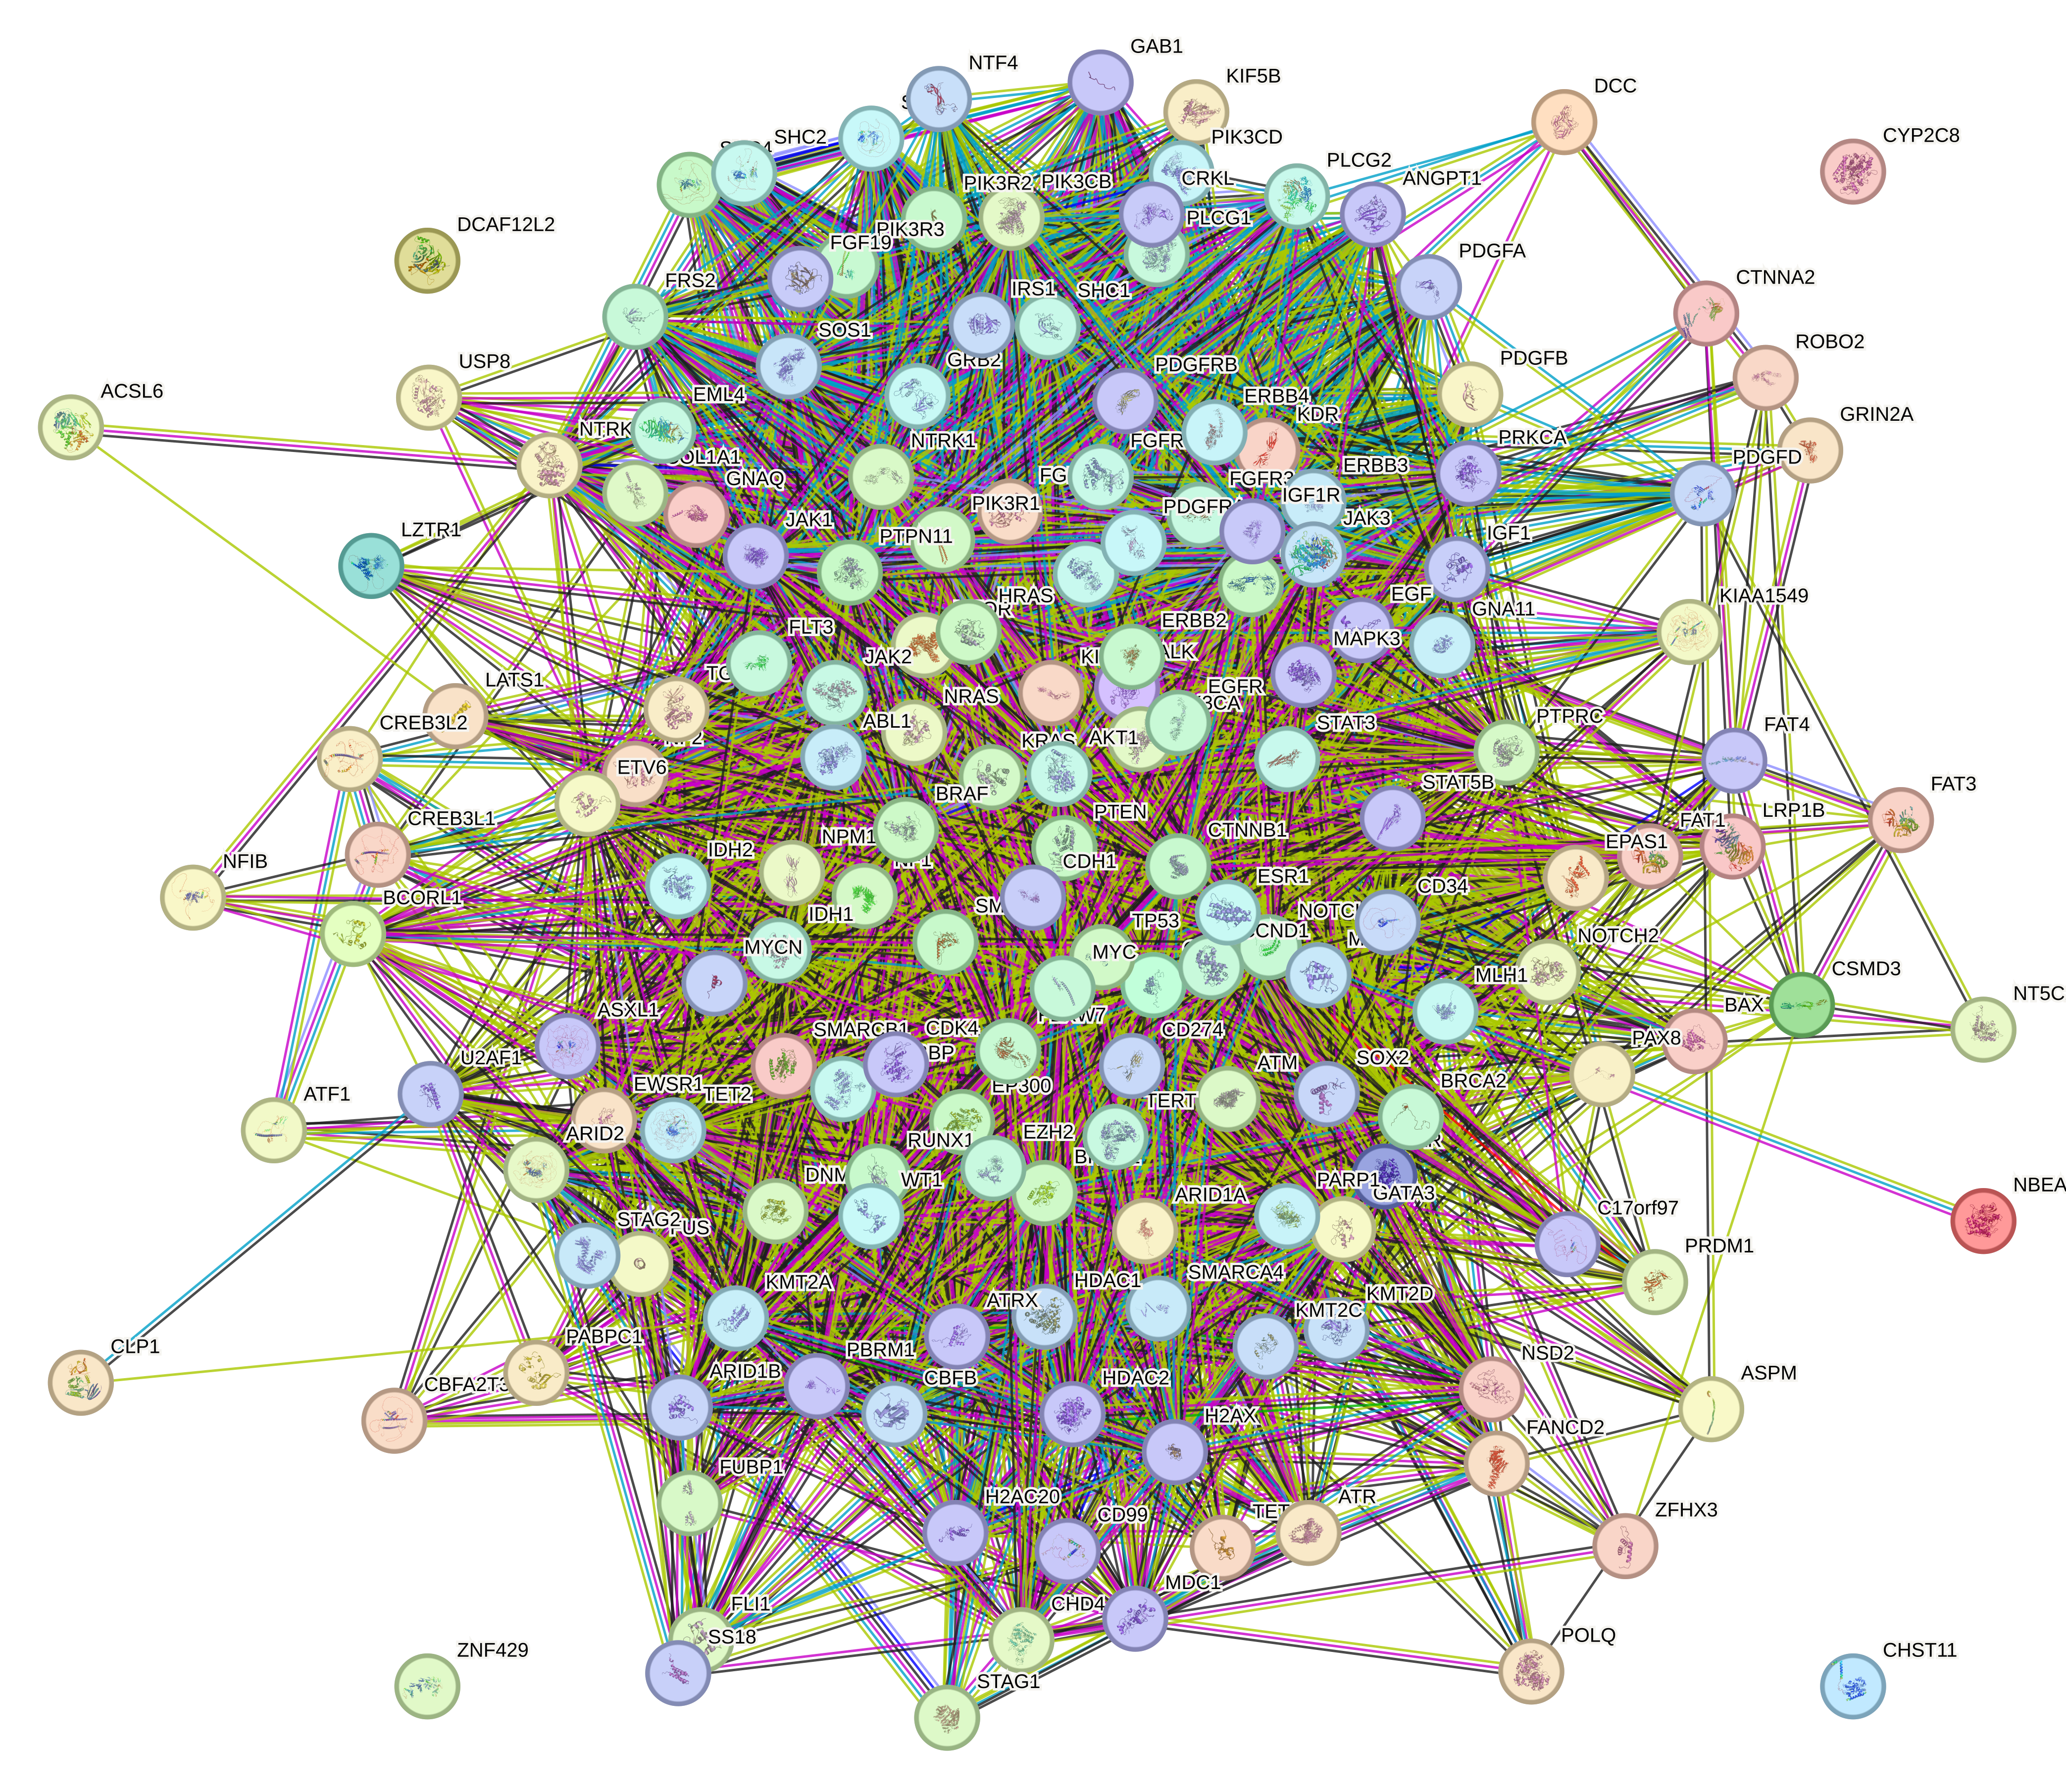
\includegraphics[width=0.95\textwidth]{figures/string_hires_image.png}
		\caption{STRING protein--protein interaction network generated from schwannoma-associated genes.}
		\label{fig:string_network}
	\end{figure}
		\begin{figure}[H]
		\centering
		\includegraphics[width=0.95\textwidth]{figures/string_gene_input.png}
		\caption{STRING multiple gene input from the results of the previous step. HGNC symbols are used in this step.}
		\label{fig:string_gene_input}
	\end{figure}
		\begin{figure}[H]
		\centering
		\includegraphics[width=0.95\textwidth]{figures/string_max_interactor_100.png}
		\caption{STRING setting max interaction to 100 according to the project description.}
		\label{fig:string_max_interaction}
	\end{figure}
	
	\subsection{Step 3: Variant Retrieval Using Ensembl BioMart}
	
	The expanded gene set obtained from STRING was converted into Ensembl Gene Stable IDs to ensure compatibility with downstream genomic queries. These Ensembl IDs were then used to retrieve genetic variants from the Ensembl BioMart \texttt{hsapiens\_snp} dataset.
	
	Variants were restricted to those originating from the dbSNP database by applying the \texttt{variation\_source = dbSNP} filter. For each gene, the following variant-related attributes were retrieved: Ensembl Gene Stable ID, gene name, dbSNP identifier, chromosome name, variant start and end positions, alleles, and UCSC genome browser identifier (when available).
	
	Due to instability and frequent timeouts when querying BioMart for large gene lists, a custom Python script was implemented to automate the querying process. The script submits XML-based BioMart queries programmatically and cycles through multiple Ensembl mirror servers to maximize query reliability.
	
	To avoid server-side failures, the gene list was divided into small chunks, with a final stable configuration of four genes per query (\texttt{CHUNK\_SIZE = 4}). Each chunk was queried sequentially, and results were appended to a unified output file. The complete variant retrieval process required approximately 20 hours to finish.
	
	Screenshots of the BioMart configuration for variant-related attributes are shown in Figure~\ref{fig:biomart_variants}.
	
	\begin{figure}[H]
		\centering
		\includegraphics[width=0.25\textwidth]{figures/biomart_variants.png}
		\caption{BioMart interface showing variant-related attribute selection for dbSNP queries.}
		\label{fig:biomart_variants}
	\end{figure}
	\subsection{Automated Variant Retrieval Script (Final Working Version)}
	\label{subsec:biomart_script_final}
	
	Because BioMart queries for variant-level data frequently failed through the web interface (timeouts, incomplete output, or session termination), we implemented a Python script that programmatically submits BioMart XML queries to Ensembl’s \texttt{martservice} endpoint. The script automates three key requirements: (1) chunking the input gene list to avoid request size/time limits, (2) retrying failed requests and rotating across multiple Ensembl mirror servers, and (3) storing each chunk result independently, then merging all chunk files into a final unified TSV output.
	
	\paragraph{Procedure (end-to-end).}
	The pipeline implemented by the script is:
	\begin{enumerate}
		\item Read the list of Ensembl Gene Stable IDs (\texttt{ENSG...}) produced from the STRING-derived gene set.
		\item Split genes into fixed-size chunks (\texttt{CHUNK\_SIZE=4}) and build a BioMart XML query for each chunk.
		\item Submit each query to BioMart using HTTP POST; on failures, retry and switch between Ensembl mirrors.
		\item Save each chunk response to its own TSV file in \texttt{chunks/}.
		\item Merge all chunk TSV files into a final output file while keeping a single header line.
		\item Track which gene IDs actually appear in returned rows and write the remaining IDs into \texttt{missing\_gene\_ids.txt}.
	\end{enumerate}
	
	\paragraph{Functionality of major methods.}
	\begin{itemize}
		\item \texttt{read\_gene\_ids()}: reads the input file and extracts only valid Ensembl gene IDs while removing duplicates.
		\item \texttt{build\_query\_xml()}: constructs the XML query specifying dataset (\texttt{hsapiens\_snp}), filters (dbSNP source and gene list), and output attributes (gene ID/name, rsID, coordinates, alleles, UCSC ID).
		\item \texttt{post\_query()}: performs an HTTP POST to a BioMart endpoint with a timeout; raises an exception on HTTP failure.
		\item \texttt{query\_with\_mirrors()}: tries multiple Ensembl mirrors and retries each mirror several times before declaring the chunk failed.
		\item \texttt{returned\_gene\_ids\_from\_tsv()}: parses returned TSV rows and collects gene IDs that appear in the first column, enabling accurate ``missing gene'' detection even when BioMart returns partial results.
		\item \texttt{write\_chunk\_file()}: writes each chunk response into a separate file to prevent losing progress after long runs.
		\item \texttt{merge\_chunk\_files()}: merges chunk outputs into a single TSV, ensuring only one header is kept even though every chunk is requested with a header.
		\item \texttt{run()}: orchestrates the entire process, cleans old chunk outputs, writes logs, and produces both final data output and missing-gene list.
	\end{itemize}
	
	\paragraph{Final code used in the project.}
	The following script is the final working version used to retrieve all dbSNP variants for the STRING-expanded schwannoma-associated gene set. In our final run, \texttt{CHUNK\_SIZE=4} produced stable requests, but the full download still required approximately 20 hours due to BioMart rate limits and intermittent failures.
	
	\begin{lstlisting}[language=Python, caption={Final working BioMart variant retrieval script (chunked, mirror-aware, merge-based).}, label={lst:biomart_final}]
		#!/usr/bin/env python3
		from __future__ import annotations
		
		import sys
		import time
		from typing import List, Tuple
		import requests
		
		# ============================================================
		# DEBUG DEFAULTS (NO TERMINAL INPUT NEEDED)
		# Edit these paths for your machine if needed.
		# ============================================================
		
		GENE_FILE = r"string_proteins_gene_stable_id_full.txt"
		OUT_TSV   = r"biomart_variants.tsv"
		OUT_MISS  = r"missing_gene_ids.txt"
		
		DATASET = "hsapiens_snp"
		CHUNK_SIZE = 4
		
		MIRRORS = [
		"https://www.ensembl.org/biomart/martservice",
		"https://uswest.ensembl.org/biomart/martservice",
		"https://useast.ensembl.org/biomart/martservice",
		"https://asia.ensembl.org/biomart/martservice",
		]
		
		# From your BioMart XML view:
		FILTER_SOURCE_NAME = "variation_source"
		FILTER_GENE_NAME   = "ensembl_gene"
		FILTER_SOURCE_VALUE = "dbSNP"
		
		ATTRIBUTES = [
		"ensembl_gene_stable_id",
		"ensembl_gene_name",
		"refsnp_id",
		"chr_name",
		"chrom_start",
		"chrom_end",
		"allele",
		"ucsc_id",
		]
		
		LOG_FILE = "run.log"
		
		def returned_gene_ids_from_tsv(tsv_text: str) -> set:
			out = set()
			for ln in tsv_text.splitlines():
				if not ln.strip():
					continue
				if ln.startswith("Gene stable ID"):  # skip header if present
					continue
				out.add(ln.split("\t", 1)[0])  # first column is gene stable id
			return out
		
		def log(msg: str) -> None:
			print(msg)
			with open(LOG_FILE, "a", encoding="utf-8", newline="\n") as f:
				f.write(msg + "\n")
		
		def read_gene_ids(path: str) -> List[str]:
			ids = []
			with open(path, "r", encoding="utf-8") as f:
				for line in f:
					s = line.strip()
					if not s:
						continue
					if s.lower().startswith("gene") or s.lower().startswith("ensembl"):
						continue
					if s.startswith("ENSG"):
						ids.append(s)
			
			seen = set()
			out = []
			for g in ids:
				if g not in seen:
					seen.add(g)
					out.append(g)
			return out
		
		def build_query_xml(dataset: str, genes: List[str], header: int = 1) -> str:
			gene_list = ",".join(genes)
			attrs = "\n".join([f'    <Attribute name = "{a}" />' for a in ATTRIBUTES])
			return f"""<?xml version="1.0" encoding="UTF-8"?>
			<!DOCTYPE Query>
			<Query virtualSchemaName = "default" formatter = "TSV" header = "{header}" uniqueRows = "1" count = "" datasetConfigVersion = "0.6" >
			<Dataset name = "{dataset}" interface = "default" >
			<Filter name = "{FILTER_SOURCE_NAME}" value = "{FILTER_SOURCE_VALUE}"/>
			<Filter name = "{FILTER_GENE_NAME}" value = "{gene_list}"/>
			{attrs}
			</Dataset>
			</Query>
			"""
		
		def post_query(mirror: str, xml: str, timeout: int = 180) -> str:
			r = requests.post(mirror, data={"query": xml}, timeout=timeout)
			r.raise_for_status()
			return r.text
		
		def is_biomart_error(txt: str) -> bool:
			low = txt.lower()
			return ("query error" in low) or ("biomart::exception" in low) or ("dataset" in low and "not found" in low)
		
		def query_with_mirrors(xml: str, retries: int = 3) -> Tuple[str, str]:
			last_err = None
			for mirror in MIRRORS:
				for attempt in range(1, retries + 1):
					try:
						txt = post_query(mirror, xml)
						if is_biomart_error(txt):
							raise RuntimeError(txt.splitlines()[0] if txt else "BioMart error")
						return txt, mirror
					except Exception as e:
						last_err = e
						time.sleep(1.2 * attempt)
			raise RuntimeError(f"All mirrors failed. Last error: {last_err}")
		
		def parse_returned_gene_ids(tsv: str) -> set:
			lines = [ln for ln in tsv.splitlines() if ln.strip()]
			if len(lines) < 2:
				return set()
			header = lines[0].split("\t")
			idx = None
			for key in ("Ensembl Gene Stable ID", "ensembl_gene_stable_id"):
				if key in header:
					idx = header.index(key)
					break
			if idx is None:
				return set()
			out = set()
			for ln in lines[1:]:
				parts = ln.split("\t")
				if len(parts) > idx:
					out.add(parts[idx])
			return out
		
		import os
		from pathlib import Path
		
		def write_chunk_file(chunk_dir: str, chunk_index: int, txt: str) -> str:
			"""
			Writes one chunk output to a separate TSV file.
			Returns the filepath.
			"""
			Path(chunk_dir).mkdir(parents=True, exist_ok=True)
			fp = os.path.join(chunk_dir, f"biomart_variants_chunk_{chunk_index:04d}.tsv")
			with open(fp, "w", encoding="utf-8", newline="\n") as f:
			f.write(txt if txt.endswith("\n") else (txt + "\n"))
			return fp
		
		def merge_chunk_files(chunk_files: List[str], out_tsv: str) -> None:
			"""
			Merges chunk TSV files into a single TSV.
			Keeps exactly ONE header (from the first chunk file that has a header).
			If chunks have no header (header=0), it merges as-is.
			"""
			# Determine if the first non-empty chunk begins with a header line
			header_line = None
			first_data_seen = False
			
			with open(out_tsv, "w", encoding="utf-8", newline="\n") as out:
				for fp in chunk_files:
					with open(fp, "r", encoding="utf-8") as f:
						lines = f.read().splitlines()
					
					# Skip completely empty chunk files
					if not any(ln.strip() for ln in lines):
						continue
					
					# If we haven't decided on a header yet, detect it
					if header_line is None:
						first_nonempty = next((ln for ln in lines if ln.strip()), "")
						if first_nonempty.startswith("Gene stable ID"):
							header_line = first_nonempty
							out.write(header_line + "\n")
							# write remaining lines excluding header
							for ln in lines[1:]:
								if ln.strip():
									out.write(ln + "\n")
							first_data_seen = True
							continue
						else:
							# No header in this file; just write all lines
							for ln in lines:
								if ln.strip():
									out.write(ln + "\n")
							first_data_seen = True
							continue
					
					# Header already known:
					if lines and lines[0].startswith("Gene stable ID"):
						# Skip the header line in subsequent chunks
						for ln in lines[1:]:
							if ln.strip():
								out.write(ln + "\n")
					else:
						for ln in lines:
							if ln.strip():
								out.write(ln + "\n")
			
			if not first_data_seen:
				# Ensure output exists but is empty if nothing was merged
				open(out_tsv, "w", encoding="utf-8").close()
		
		def run():
		import os
		
		# reset log
		open(LOG_FILE, "w", encoding="utf-8").close()
		
		log(f"Using dataset={DATASET}")
		log(f"Gene file: {GENE_FILE}")
		log(f"Output TSV: {OUT_TSV}")
		log(f"Chunk size: {CHUNK_SIZE}")
		
		gene_ids = read_gene_ids(GENE_FILE)
		if not gene_ids:
			log("ERROR: No ENSG IDs found in input file.")
			sys.exit(1)
		
		log(f"Input genes: {len(gene_ids)}")
		log(f"First 3 gene IDs: {gene_ids[:3]}")
		
		# Directory to store chunk results
		chunk_dir = "chunks"
		
		# Clean old chunk files (avoid mixing old + new)
		if os.path.isdir(chunk_dir):
			for fn in os.listdir(chunk_dir):
				if fn.startswith("biomart_variants_chunk_") and fn.endswith(".tsv"):
					try:
						os.remove(os.path.join(chunk_dir, fn))
					except Exception:
						pass
		else:
			os.makedirs(chunk_dir, exist_ok=True)
		
		returned_genes_all = set()
		chunk_files: List[str] = []
		failed_chunks: List[int] = []
		
		# We will request header=1 for EVERY chunk file.
		# Reason: simplifies merge + missing gene detection.
		# We will remove duplicate headers at merge time.
		for idx, i in enumerate(range(0, len(gene_ids), CHUNK_SIZE), start=1):
			chunk_genes = gene_ids[i:i + CHUNK_SIZE]
			xml = build_query_xml(DATASET, chunk_genes, header=1)
			
			# keep last query for debugging
			with open("last_query.xml", "w", encoding="utf-8") as f:
				f.write(xml)
			
			try:
				txt, used = query_with_mirrors(xml)
				log(f"Chunk {idx}: genes {i+1}-{min(i+CHUNK_SIZE, len(gene_ids))} OK (mirror: {used})")
				log(f"Response length: {len(txt)} chars")
				
				# Save this chunk output separately
				fp = write_chunk_file(chunk_dir, idx, txt)
				chunk_files.append(fp)
				
				# Update returned genes set from the real returned TSV text
				returned_genes_all |= returned_gene_ids_from_tsv(txt)
			
			except Exception as e:
				failed_chunks.append(idx)
				log(f"ERROR: Chunk {idx} failed. Reason: {e}")
			
			time.sleep(0.4)
		
		# Merge chunk files into final output
		if chunk_files:
			merge_chunk_files(chunk_files, OUT_TSV)
			try:
			size = __import__("os").path.getsize(OUT_TSV)
			log(f"Final merged TSV size: {size} bytes")
			except Exception as e:
			log(f"Could not stat merged output TSV: {e}")
		else:
			# no chunks succeeded
			open(OUT_TSV, "w", encoding="utf-8").close()
			log("WARNING: No chunk files produced. Output TSV is empty.")
		
		# Missing genes = those never observed in returned data
		missing = [g for g in gene_ids if g not in returned_genes_all]
		with open(OUT_MISS, "w", encoding="utf-8", newline="\n") as f:
			f.write("\n".join(missing) + ("\n" if missing else ""))
		
		log(f"Genes with no returned rows: {len(missing)} -> {OUT_MISS}")
		if failed_chunks:
			log(f"Failed chunks: {failed_chunks} (you can re-run; successful chunks are preserved in {chunk_dir}/)")
		log("DONE.")
		
		
		if __name__ == "__main__":
			run()
		
	\end{lstlisting}
	
	
	% =========================================================
\section{Part 3: Genomic Coordinates and Transcript Annotation}

In this part, genomic coordinates and transcript-level structural information were retrieved for the genes identified in Part~2. Since the STRING database gene list was converted to Ensembl Gene IDs, and UCSC RefSeq tables are transcript-centric, we adopted a transcript-level representation in order to preserve all available annotation without introducing arbitrary transcript selection criteria.
\begin{figure}[H]
	\centering
	\includegraphics[width=\textwidth]{figures/ucsc_table_browser_setup.png}
	\caption{UCSC Table Browser configuration showing genome assembly (hg38), RefSeq track, and ncbiRefSeq table selection.}
	\label{fig:ucsc_table_browser_setup}
\end{figure}

\begin{figure}[H]
	\centering
	\includegraphics[width=0.9\textwidth]{figures/ucsc_field_selection.png}
	\caption{Selection of transcript-level fields from the hg38.ncbiRefSeq table, including genomic coordinates and exon structure.}
	\label{fig:ucsc_field_selection}
\end{figure}

\begin{figure}[H]
	\centering
	\includegraphics[width=0.9\textwidth]{figures/ucsc_identifier_input.png}
	\caption{Input of gene symbols into the UCSC Table Browser identifier field for RefSeq-based transcript retrieval.}
	\label{fig:ucsc_identifier_input}
\end{figure}

\subsection{Data Source and Genome Assembly}

Genomic annotations were obtained using the \textbf{UCSC Table Browser}. All queries were performed on the human genome assembly \textbf{GRCh38 (hg38)}. The following configuration was used consistently throughout this step:
\begin{itemize}
	\item Clade: Mammal
	\item Genome: Human
	\item Assembly: GRCh38 (hg38)
	\item Group: Genes and Gene Predictions
	\item Track: NCBI RefSeq
	\item Table: \texttt{ncbiRefSeq}
\end{itemize}

Figure~\ref{fig:ucsc_table_browser_setup} shows the Table Browser configuration used to select the appropriate dataset and genome assembly.

\subsection{Input Identifiers}

Gene symbols corresponding to the Ensembl Gene IDs obtained in Part~2 were used as input identifiers. These symbols were pasted directly into the \emph{Identifiers (names/accessions)} field of the UCSC Table Browser. The \texttt{ncbiRefSeq} table accepts gene symbols and RefSeq transcript accessions through its primary and alias tables, enabling successful mapping for the majority of genes.

An example of the identifier input interface is shown in Figure~\ref{fig:ucsc_identifier_input}.

\subsection{Selected Attributes}

To comprehensively capture transcript-level genomic structure, the following fields were selected from the \texttt{hg38.ncbiRefSeq} table:
\begin{itemize}
	\item \texttt{name} (RefSeq transcript accession)
	\item \texttt{chrom} (chromosome)
	\item \texttt{strand}
	\item \texttt{txStart}, \texttt{txEnd} (transcription start and end positions)
	\item \texttt{exonCount}
	\item \texttt{exonStarts}
	\item \texttt{exonEnds}
	\item \texttt{name2} (gene symbol)
\end{itemize}

These fields provide both gene-level identifiers and detailed exon–intron structure for each transcript. Figure~\ref{fig:ucsc_field_selection} illustrates the field selection interface used in this step.

\subsection{Transcript-Level Representation}

The UCSC RefSeq table returns multiple transcript entries for many genes, including protein-coding (e.g., \texttt{NM\_}, \texttt{XM\_}) and non-coding (e.g., \texttt{NR\_}, \texttt{XR\_}) transcripts. Rather than selecting a single representative transcript per gene, all returned transcripts were retained.

This design choice ensures:
\begin{itemize}
	\item no loss of structural information,
	\item compatibility with alternative splicing analysis,
	\item transparent linkage between gene symbols and multiple transcript isoforms.
\end{itemize}

Each transcript is uniquely identified by its RefSeq accession and linked to the corresponding gene symbol via the \texttt{name2} field.

\subsection{Output Format and Downstream Use}

The resulting data were exported in tab-separated (TSV) format and later imported into a relational database. Each row corresponds to a single RefSeq transcript, with exon boundaries stored as comma-separated coordinate lists.

This transcript-level table serves as the genomic backbone for subsequent project components, enabling joins with variant data (Part~2) and protein-level annotations in later stages of the project.

\section{Part 4 — UniProt ID Mapping (Genes $\rightarrow$ Proteins)}\label{sec:uniprot}
I got the Ensembl Gene IDs from the previous part and used the UniProt website to map them to UniProt IDs.
\begin{figure}[H]
	\centering
	\includegraphics[width=0.9\textwidth]{figures/ID_mapping.png}
	\caption{ID mapping interface showing the mapping of Ensembl Gene IDs to UniProt IDs.}
	\label{fig:id_mapping}
\end{figure}

Then I downloaded the data and saved it in a `idmapping.tsv` TSV file.
Fortunately, there were not any missing genome that has not protein. and as mentioned in the documentation the columns are added.

	% =========================================================
	\section{Part 5 — GEO Dataset \& GEO2R}\label{sec:geo}
	Describe GEO search constraints (human, since Jan 1 2005), chosen dataset, and the GEO2R output table.
	
	% =========================================================
	\section{Part 6 — Additional Table from Another Database}\label{sec:extra}
	Add at least one additional table and explain how it links (or add a cross-reference table).
	
	% =========================================================
	\section{Part 7 — Conceptual Design (ER Diagram + Keys)}\label{sec:er}
	\subsection{Entity-Relationship diagram}
	%\begin{figure}[htbp]
	%	\centering
	%	\includegraphics[width=0.95\linewidth]{figures/er_diagram.pdf}
	%	\caption{\textbf{ER diagram of the Schwannoma database.} Cardinalities are shown on relationships.}
	%	\label{fig:er}
	%\end{figure}
	
	\subsection{Primary keys and foreign keys}
	List PK/FK per table (you can use bullets or a small table).
	
	% =========================================================
	\section{Challenges and Ambiguities}\label{sec:challenges}
		
	\subsection{Code Evolution and Rationale (Old vs. New Implementation)}
	\label{subsec:code_evolution}
	
	During Part 2, we iteratively improved the variant-retrieval code as repeated failures appeared when scaling from small test gene lists to the full STRING-expanded set. The core difficulties were BioMart instability (timeouts, truncated responses such as ``Response ended prematurely''), long runtimes, and incorrect missing-gene reporting when the returned output was incomplete.
	
	\paragraph{Old implementation (direct append approach).}
	The earlier version of the script appended each chunk response directly into the final TSV file as the run progressed, and it tracked missing genes using a header-dependent parsing strategy that effectively only validated the first chunk. This older strategy was workable for very small gene lists but was fragile when the service intermittently failed.
	
	\textbf{Drawbacks of the old approach:}
	\begin{itemize}
		\item \textbf{Progress was not safely checkpointed:} if a late chunk failed after many hours, there was no reliable way to resume without re-running everything.
		\item \textbf{Missing-gene detection was inaccurate:} the code only accumulated returned gene IDs from the first chunk (the only chunk guaranteed to include the header), causing many genes to be incorrectly written into \texttt{missing\_gene\_ids.txt} even when their variants existed in later chunks.
		\item \textbf{Hard to debug partial results:} all outputs were mixed into one file, so identifying which chunk caused corruption or truncation was difficult.
	\end{itemize}
	
	\paragraph{Old code used before the final fix.}
	\begin{lstlisting}[language=Python, caption={Old BioMart variant retrieval script (single output append, fragile missing-gene tracking).}, label={lst:biomart_old}]
		def run():
			# reset log
			open(LOG_FILE, "w", encoding="utf-8").close()
			
			log(f"Using dataset={DATASET}")
			log(f"Gene file: {GENE_FILE}")
			log(f"Output TSV: {OUT_TSV}")
			log(f"Chunk size: {CHUNK_SIZE}")
			
			gene_ids = read_gene_ids(GENE_FILE)
			if not gene_ids:
				log("ERROR: No ENSG IDs found in input file.")
				sys.exit(1)
			
			log(f"Input genes: {len(gene_ids)}")
			log(f"First 3 gene IDs: {gene_ids[:3]}")
			
			# reset outputs
			open(OUT_TSV, "w", encoding="utf-8").close()
			
			header_written = False
			returned_genes_all = set()
			
			for i in range(0, len(gene_ids), CHUNK_SIZE):
				chunk_genes = gene_ids[i:i + CHUNK_SIZE]
				
				# header=1 only for first chunk; then header=0
				xml = build_query_xml(DATASET, chunk_genes, header=1 if not header_written else 0)
				
				# For debugging: write the XML being sent
				with open("last_query.xml", "w", encoding="utf-8") as f:
				f.write(xml)
				
				txt, used = query_with_mirrors(xml)
				log(f"Chunk {i//CHUNK_SIZE + 1}: genes {i+1}-{min(i+CHUNK_SIZE, len(gene_ids))} OK (mirror: {used})")
				log(f"Response length: {len(txt)} chars")
				
				with open(OUT_TSV, "a", encoding="utf-8", newline="\n") as f:
				f.write(txt if txt.endswith("\n") else (txt + "\n"))
				
				# track returned genes from first chunk only (has header)
				if not header_written:
				returned_genes_all |= parse_returned_gene_ids(txt)
				header_written = True
				
				time.sleep(0.4)
			
			# If TSV is empty, log it explicitly
			try:
				size = __import__("os").path.getsize(OUT_TSV)
				log(f"Final TSV size: {size} bytes")
				if size < 5:
					log("WARNING: TSV file is essentially empty. Check last_query.xml and run.log.")
			except Exception as e:
				log(f"Could not stat output TSV: {e}")
			
			missing = [g for g in gene_ids if g not in returned_genes_all]
			with open(OUT_MISS, "w", encoding="utf-8", newline="\n") as f:
				f.write("\n".join(missing) + ("\n" if missing else ""))
			
			log(f"Genes not observed in first-chunk tracking: {len(missing)} -> {OUT_MISS}")
			log("DONE.")
	\end{lstlisting}
	
	\paragraph{New implementation (chunk files + merge + accurate tracking).}
	To address these issues, we redesigned the script around \textbf{checkpointed chunk files}. Each chunk is written into a separate TSV file under \texttt{chunks/}. This makes the pipeline resilient: if BioMart fails mid-run, successful chunks remain saved and can be reused without recomputing earlier results. Additionally, the new implementation requests a header for every chunk (\texttt{header=1}) and removes duplicate headers during the merge step. This greatly simplifies debugging and allows consistent parsing.
	
	The ``missing genes'' list is now computed from the actual returned rows across \emph{all} chunk outputs using \texttt{returned\_gene\_ids\_from\_tsv()}, which does not rely on the presence of a header or a specific column index.
	
	\textbf{Advantages of the new approach:}
	\begin{itemize}
		\item \textbf{Checkpointing:} intermediate results persist even if the run takes many hours.
		\item \textbf{Correct missing-gene reporting:} genes are marked missing only if they never appear in any returned row across all chunks.
		\item \textbf{Traceability:} errors can be linked to a specific chunk file and re-run strategy can focus only on failed indices.
		\item \textbf{Stable merging:} output is normalized into one TSV with a single header.
	\end{itemize}
	
	This final version (Section~\ref{subsec:biomart_script_final}) successfully completed the full variant download with \texttt{CHUNK\_SIZE=4}, producing a comprehensive variant dataset, although the total runtime was approximately 20 hours due to service constraints and enforced throttling.
	
	
	% =========================================================
	% Single-file bibliography:
	% Add items as you go; keep keys stable, cite with \cite{key}.
	\begin{thebibliography}{99}
		
	\bibitem{review_schwannoma_2020}
	Plotkin, S. R., \& Asthagiri, A. R.
	\newblock Schwannoma and vestibular schwannoma.
	\newblock \emph{The Lancet Oncology}, 21(7), e349--e359, 2020.
	
	\bibitem{vestibular_epidemiology_2019}
	Carlson, M. L., et al.
	\newblock Epidemiology of vestibular schwannoma.
	\newblock \emph{Otolaryngologic Clinics of North America}, 52(4), 607--620, 2019.
	
	\bibitem{omim_nf2}
	OMIM.
	\newblock Neurofibromatosis type 2 (NF2), OMIM Entry \#101000.
	\newblock \url{https://omim.org/entry/101000}
	
	\bibitem{pathology_schwannoma_2018}
	Rodriguez, F. J., et al.
	\newblock Pathology of peripheral nerve sheath tumors.
	\newblock \emph{Acta Neuropathologica}, 135(1), 1--19, 2018.
	
	\bibitem{merlin_signaling_2021}
	Li, W., \& Cooper, J.
	\newblock The tumor suppressor merlin and its role in NF2-associated tumors.
	\newblock \emph{Nature Reviews Cancer}, 21, 593--610, 2021.
	
	\bibitem{genomics_schwannoma_2022}
	Agnihotri, S., et al.
	\newblock Genomic and epigenomic landscape of schwannomas.
	\newblock \emph{Nature Communications}, 13, 1842, 2022.
	
	\bibitem{merlin_signaling_2024}
	Duo Xu, Shiyuan Yin \& Yongqian Shu
	\newblock NF2: An underestimated player in cancer metabolic reprogramming and tumor immunity.
	\newblock \emph{npj Precision Oncology}, 2024.
	
	\bibitem{FernandezMendez2023}
	R.~Fernández-Méndez, Y.~Wan, P.~Axon, and A.~Joannides,
	``Incidence and presentation of vestibular schwannoma: a 3-year cohort registry study,''
	\emph{Acta Neurochirurgica}, vol.~165, no.~10, pp.~2903--2911, 2023.
	doi:10.1007/s00701-023-05665-9.
	
	\bibitem{Price2024CBTRUS}
	M.~Price \emph{et al.},
	``CBTRUS Statistical Report: Primary Brain and Other Central Nervous System Tumors Diagnosed in the United States in 2017--2021,''
	\emph{Neuro-Oncology}, vol.~26, Suppl.~6, pp.~vi1--vi85, 2024.
	doi:10.1093/neuonc/noae145.
		
		\bibitem{string_db}
		STRING Consortium.
		\newblock STRING database: known and predicted protein-protein interactions.
		\newblock Accessed: Jan 2026.
		
		\bibitem{ensembl_biomart}
		Ensembl.
		\newblock Ensembl BioMart.
		\newblock Accessed: Jan 2026.
		
		\bibitem{ucsc_table_browser}
		UCSC Genome Browser.
		\newblock UCSC Table Browser tool documentation.
		\newblock Accessed: Jan 2026.
		
		\bibitem{uniprot}
		UniProt Consortium.
		\newblock UniProt: the universal protein knowledgebase.
		\newblock Accessed: Jan 2026.
		
		\bibitem{geo}
		NCBI.
		\newblock Gene Expression Omnibus (GEO) and GEO2R.
		\newblock Accessed: Jan 2026.
		
	\end{thebibliography}
	
\end{document}
